% Baccalauréat malgache, série C, 2008 : énoncé.
\TCDBacAttribution{C}{2008}
\providecommand{\dx}{\mathrm{d}x}
\providecommand{\Re}[1]{\mathrm{Re}\left( #1 \right)}
\providecommand{\Im}[1]{\mathrm{Im}\left( #1 \right)}
\providecommand{\dt}{\mathrm{d}t}
\providecommand{\Ouv}{(O;\vec{u},\vec{v})}
\providecommand{\mes}[2]{\mathrm{mes}\left( \widehat{ \overrightarrow{#1} ; \overrightarrow{#2} } \right)}
\providecommand{\D}{(\mathscr{D})}
\providecommand{\Courbe}{(\mathscr{C})}
\providecommand{\Courben}{(\mathscr{C}_n)}
\providecommand{\CourbeD}{(\mathscr{C}_2)}
\providecommand{\congru}[3]{#1 \equi #2 \quad \left[ \mathrm{mod}~#3\right]}
%
%%%%%%%%%%%%%%%%%%%%%%%%%%%%%%%%%%%%%%%%%%%%%%%%%%%%%%%%%%%%%%%%%%%%%%%%%%%%%%%%%%%%%%%%%%%%%%%%%%%%%%%%%%%%%%%%%%%%%%%%%%%%%%%%
\noindent \underline{\textsc{\textbf{Exercice}}} (4 points) 
      \begin{description}
            \item[A- Probabilit\'e]~\newline
                  Une urne contient six billes indiscernables au toucher, dont quatre num\'erot\'ees 12 et deux num\'erot\'ees 13.
                  \begin{enumerate}
                        \item Pour commencer, le jeu consiste \`a extraire simultan\'ement et au hasard trois billes de l'urne.
                              Calculer la probabilit\'e de chacun des \'ev\`enements suivants :
                              \begin{itemize}
                                    \item $E$ : << La somme des trois nombres inscrits sur les trois billes extraites est
                                                   strictement sup\'erieure \`a 36 >>.
                                    \item $F$ : << Les trois billes extraites portent le m\^eme num\'ero >>.
                              \end{itemize}
                        \item Maintenant, le jeu consiste \`a extraire successivement et sans remise, deux billes de l'urne.
                              Calculer la probabilit\'e de l'\'ev\`enement :
                              \begin{itemize}
                                    \item $G$ : << Le produit des deux nombres inscrits sur les deux billes est 
                                                   un carr\'e parfait >>.
                              \end{itemize}
                        \item Enfin, le jeu consiste \`a extraire successivement et avec remise, sept billes de l'urne.
                              Calculer la probabilit\'e de l'\'ev\`enement :
                              \begin{itemize}
                                    \item $H$ : << Obtenir au moins une bille num\'ero 13 >>.
                              \end{itemize}
                  \end{enumerate}
                  \begin{center}
                        \underline{N.B :} On donnera tous les r\'esultats \`a $10^{-2}$ pr\`es.
                  \end{center}
            \item[B- Arithm\'etique]
                  \begin{enumerate}
                        \item On consid\`ere le nombre $A$ d\'efini pour tout entier naturel $n$ par $A = 9^{n+1} + 2^{6n+1}$.
                              D\'emontrer que $A$ est divisible par $11$ pour tout $n$ de $\mathbb{N}$ :
                              \begin{enumerate}
                                    \item en utilisant les congruences.
                                    \item en raisonnant par r\'ecurrence.
                              \end{enumerate}
                        \item D\'eterminer tous les entiers relatifs $x$ v\'erifiant le syst\`eme :
                              \[
                                    \begin{multiform}
                                          \congru{3x-2}{0}{5} \\
                                          |x| < 10 \;.
                                    \end{multiform}
                              \]
                  \end{enumerate}
      \end{description}
%%%%%%%%%%%%%%%%%%%%%%%%%%%%%%%%%%%%%%%%%%%%%%%%%%%%%%%%%%%%%%%%%%%%%%%%%%%%%%%%%%%%%%%%%%%%%%%%%%%%%%%%%%%%%%%%%%%%%%%%%%%%%%%%
\noindent \underline{\textsc{\textbf{PROBLEME I}}} (7 points) 
      \begin{description}
            \item[Partie A]~\par 
                  \begin{minipage}{0.65\actualtextwidth}
                        Dans le plan orient\'e $\Plan$, l'unit\'e de longueur est le centim\`etre.
                        On donne :
                        \begin{itemize}
                              \item Le triangle $OAB$ (figure ci-contre).
                              \item Le triangle $OCB$, \'equilat\'eral direct de centre de gravit\'e $G$.
                              \item $R_B$ la rotation de centre $B$ et d'angle $\frac{\pi}{3}$.
                              \item $R_O$ la rotation de centre $O$ et d'angle $\frac{\pi}{3}$.
                              \item $R$ la compos\'ee $R_B \circ R_O$.
                        \end{itemize}
                  \end{minipage}
                  %
                  \begin{minipage}{0.25\actualtextwidth}
                        \begin{flushright}
                              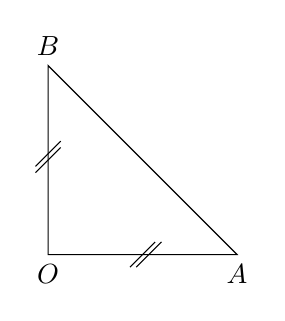
\begin{tikzpicture}[scale=.8]
                                    \draw (0,0) node[below] {$O$} -- (3,0) node[below] {$A$} -- (0,3) node[above] {$B$} -- cycle ;
                                    \draw (1.3,-.2) -- (1.7,0.2) (1.4,-.2) -- (1.8,0.2);
                                    \draw (-.2,1.3) -- (0.2,1.7) (-.2,1.4) -- (0.2,1.8);
                              \end{tikzpicture}
                        \end{flushright}
                  \end{minipage}
            \begin{enumerate}
                  \item \begin{enumerate}
                              \item Faire une figure en prenant $OA = OB = 8$.
                              \item Pr\'eciser la nature de la transformation $R$.
                              \item En d\'ecomposant $R_B$ et $R_O$, d\'eterminer le centre de $R$.
                        \end{enumerate}
                  \item On d\'esigne par $H$ le barycentre des points pond\'er\'es $(O,2)$, $(B,1)$ et $(C,1)$.
                        Soit $I$ le milieu du segment $[CB]$.
                        \begin{enumerate}
                              \item Construire $H$.
                              \item D\'eterminer l'ensemble $\Courbe$ des points $M$ du plan $\Plan$ tels que : 
                                    $ 2 \overrightarrow{MO}^2 + \overrightarrow{MC}^2 + \overrightarrow{MB}^2 
                                          = 2 \overrightarrow{AO}^2 $.
                              \item Montrer que $\Courbe$ passe par $I$.
                                    Construire $\Courbe$.
                        \end{enumerate}
            \end{enumerate}
            %
            \item[Partie B] 
                  On munit le plan $\Plan$ du rep\`ere orthonorm\'e direct $(O ; \overrightarrow{OA} , \overrightarrow{OB})$.
                  \begin{enumerate}
                        \item D\'eterminer l'affixe de chacun des points $O$, $A$, $B$, $C$ et $G$.
                        \item \begin{enumerate}
                                    \item Donner une mesure de l'angle $(\overrightarrow{OG} , \overrightarrow{OA})$
                                          et la valeur du rapport $\frac{OA}{OG}$.
                                    \item En d\'eduire les \'el\'ements caract\'eristiques de la similitude plane directe $S$
                                          qui transforme $G$ en $A$ et laisse $O$ invariant.
                                    \item Donner l'expression complexe de $S$.
                              \end{enumerate}
                  \end{enumerate}
      \end{description}
%%%%%%%%%%%%%%%%%%%%%%%%%%%%%%%%%%%%%%%%%%%%%%%%%%%%%%%%%%%%%%%%%%%%%%%%%%%%%%%%%%%%%%%%%%%%%%%%%%%%%%%%%%%%%%%%%%%%%%%%%%%%%%%%
\noindent \underline{\textsc{\textbf{PROBLEME II}}} (9 points) 
      \begin{description}
            \item[Partie A]
                  Soit $n\in\mathbb{N}^*$.
                  $f_n$ est la fonction num\'erique d\'efinie dans l'intervalle $[0;+\infty[$ par : 
                  \[
                        \begin{multiform}
                              f_n (0) = 0 \\
                              f_n (x) = x \expo{ - \frac{1}{nx} } \text{ pour } x > 0 \;.
                        \end{multiform}
                  \]
                  $\Courben$ d\'esigne la courbe repr\'esentative de $f_n$ dans un plan $\Plan$ muni d'un rep\`ere orthonorm\'e
                  direct \Oij{} d'unit\'e graphique $2\cm$.
                  \begin{enumerate}
                        \item \begin{enumerate}
                                    \item Montrer que $f_n$ est continue et d\'erivable en $O$.
                                    \item Dresser le tableau de variation de $f_n$ sur $[0;+\infty[$.
                              \end{enumerate}
                        \item On consid\`ere la fonction num\'erique $g$ d\'efinie sur $[0;+\infty[$ par 
                              $g(u) = \expo{-u} + u - 1$.
                              \begin{enumerate}
                                    \item D\'eterminer le sens de variation de $g$ sur $[0;+\infty[$.
                                    \item D\'eduire de cette monotonie de $g$, que pour tout r\'eel $u$ de $[0;+\infty[$ :
                                          $0 \leq 1 - \expo{-u} \leq u$.
                                    \item Montrer ensuite que pour tout r\'eel $h$ de $[0;+\infty[$ : 
                                          $0 \leq \expo{-h} + h - 1 \leq \frac{h^2}{2}$.
                                    \item En d\'eduire que pour tout r\'eel $x$ de $]0;+\infty[$ : 
                                          $0 \leq f_n (x) - \left( x - \frac{1}{n} \right) \leq \frac{1}{2 \ n^2 \ x}$
                                          et que la droite $(\Delta_n)$ d'\'equation $y = x - \frac{1}{n}$ est une 
                                          asymptote de $\Courben$.
                                    \item V\'erifier que $\Courben$ reste au dessus de $(\Delta_n)$.
                              \end{enumerate}
                        \item Tracer $\CourbeD$ et $(\Delta_2)$ dans $\Plan$.
                  \end{enumerate}
            \item[Partie B]
                  On pose $I_n = \int_{0}^{1} f_n (t) \dt$ pour tout entier naturel $n$ sup\'erieur ou \'egal \`a $1$.
                  \begin{description}
                        \item a) 
                              Montrer que pour tout r\'eel $t$ de $[0;1]$ : $\left(t-\frac{1}{n}\right) \leq f_n (t) \leq t$.
                        \item b) 
                              En d\'eduire que $\displaystyle{ \lim_{n\rightarrow +\infty} I_n = \frac{1}{2}}$.
                  \end{description}
            \item[Partie C]
                  On consid\'ere l'\'equation diff\'erentielle $(E)$ : $y' - y = \frac{-x^2 + x + 1}{x} \expo{-\frac{1}{x}}$.
                  \begin{enumerate}
                        \item R\'esoudre l'\'equation diff\'erentielle $(E')$ : $y' - y = 0$.
                        \item \begin{enumerate}
                                    \item Montrer que la fonction $f$ telle que $f(x) = x \expo{-\frac{1}{x}}$, o\`u 
                                          $x \in ]0;+\infty[$ est solution de $(E)$.
                                    \item $\varphi$ \'etant une fonction num\'erique d\'erivable sur $]0;+\infty[$,
                                          montrer que $(\varphi + f)$ est solution de $(E)$ si et seulement si $\varphi$ 
                                          est solution de $(E')$.
                                    \item Achever la r\'esolution de $(E)$.
                              \end{enumerate}
                  \end{enumerate}
      \end{description}
%%%%%%%%%%%%%%%%%%%%%%%%%%%%%%%%%%%%%%%%%%%%%%%%%%%%%%%%%%%%%%%%%%%%%%%%%%%%%%%%%%%%%%%%%%%%%%%%%%%%%%%%%%%%%%%%%%%%%%%%%%%%%%%%





































